\documentclass{ohm_project_description}

\projecttitle{Greifen von bewegten Objekten}
\projectauthor{Labor für mobile Robotik}
\projectdate{2025}

\begin{document}

\maketitle
\thispagestyle{fancy}

\vspace*{-2.5cm}
\begin{figure}[h!]
    \centering
    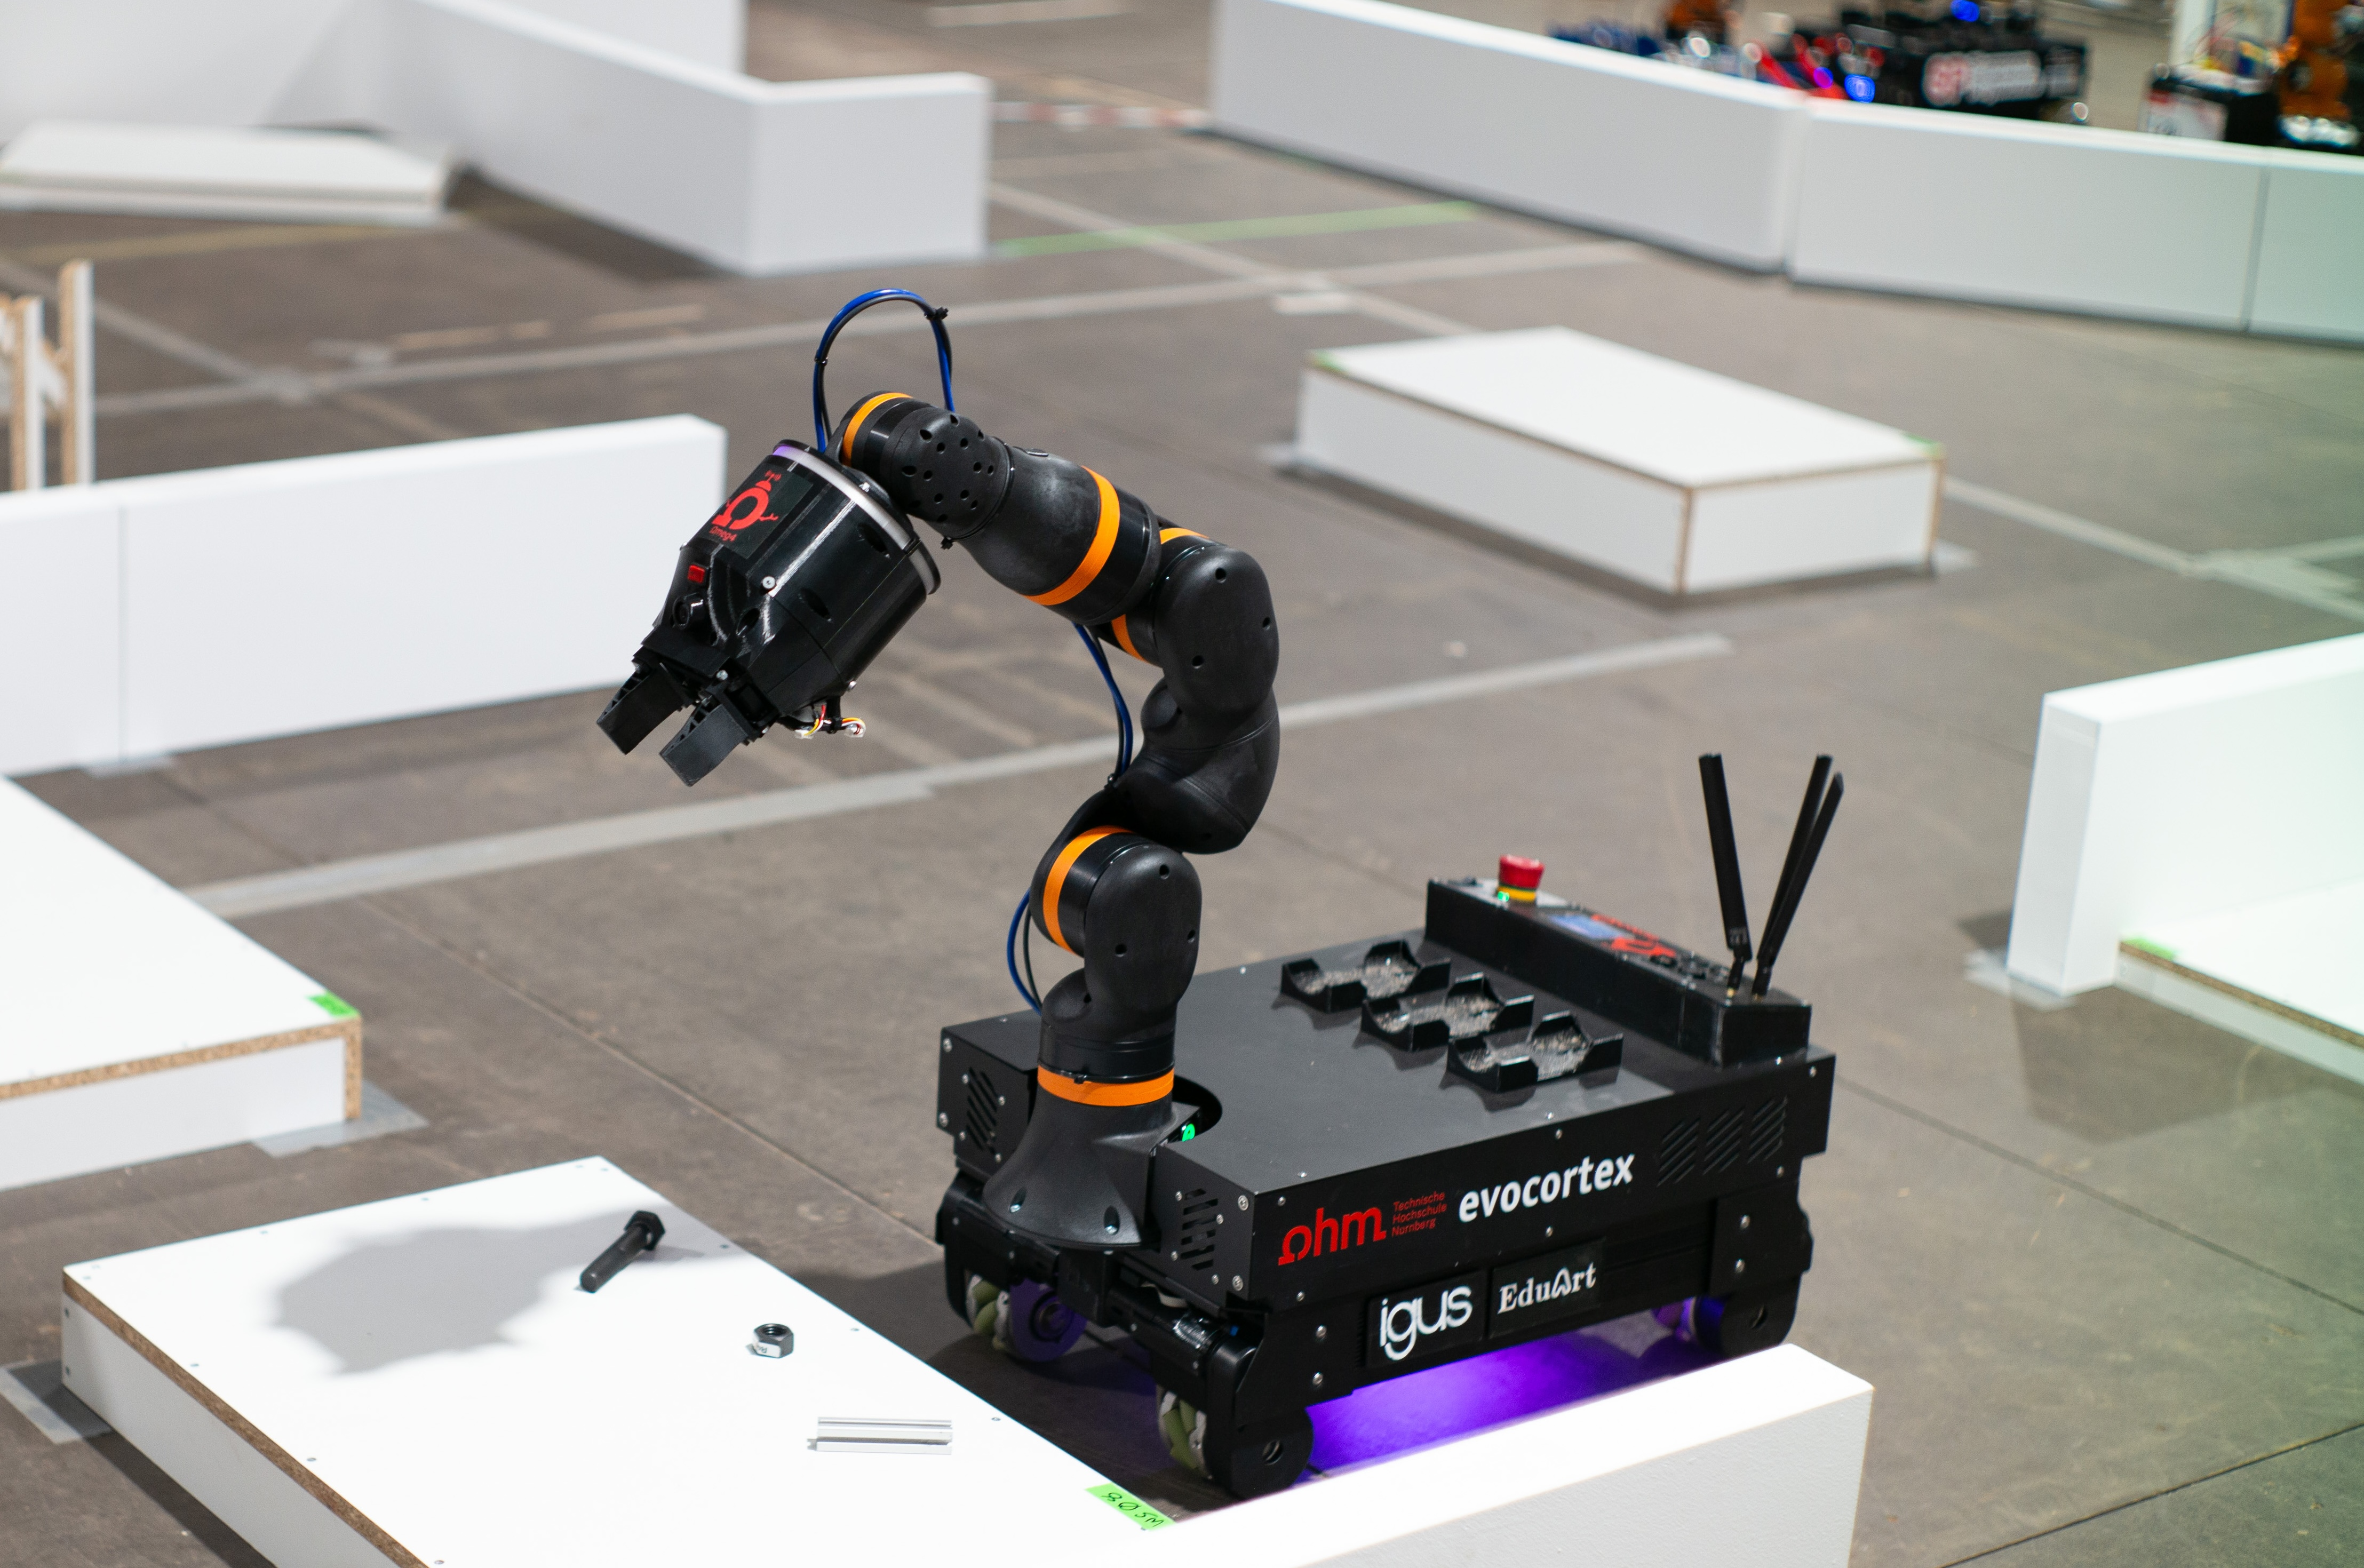
\includegraphics[height=4cm]{img/atwork.jpg}
\end{figure} 


Das Team \textbf{AutonOhm} des Labors für Mobile Robotik nimmt seit vielen Jahren erfolgreich am RoboCup Industrial @Work Wettbewerb teil. Ziel dieses Wettbewerbs ist es, einen mobilen Roboter zu entwickeln, der sich selbstständig in einer Arena zurechtfindet und vordefinierte Aufgaben der Form "Transportiere Gegenstand A von Tisch B zu Tisch C" durchführt. Für diese Aufgaben ist ein komplexes Gesamtsystem aus \emph{Lokalisierung}, \emph{Wahrnehmung}, \emph{Planung} und \emph{Steuerung} notwendig. Es bietet daher für interessierte Studierende neben einer Vielzahl von spannenden Themen im Bereich der mobilen Robotik auch die Möglichkeit, praxisnah an einem \emph{echten} Robotersystem zu arbeiten.

Im Rahmen des Wettbewerbs müssen Objekte von einer rotierenden Tischplatte gegriffen werden. Der Roboter muss daher die Bewegung der Tischplatte erkennen und die Objektpositionen entsprechend in die Zukunft predizieren. Dann muss eine geeignete Arm- und Greifpose berechnet werden, um das bewegte Objekt zu greifen. Ziel der Arbeit ist es, eine Lösung für dieses Problem zu entwickeln.  

Engagement und Mitarbeit im studentischen Team Autonohm sind ausdrücklich erwünscht! Es besteht die Möglichkeit, im Rahmen der Arbeit an nationalen und internationalen Wettbewerben teilzunehmen.

\section*{Arbeitspakete}
\begin{itemize}[leftmargin=0.5cm]
    \setlength\itemsep{.1em}
    \item Einarbeiten in die aktuelle Systemarchitektur des @Work Roboters
    \item Recherche und Implementierung eines Algorithmus für das Tracking von bewegten Objekten
    \item Recherche und Implementierung eines Algorithmus zur Berechnung von Greifposen von bewegten Objekten
    \item Integration und Demonstration auf dem Robotersystem 
\end{itemize}

\section*{Voraussetzungen}
\begin{itemize}[leftmargin=0.5cm]
    \setlength\itemsep{.1em}
    \item Grundkenntnisse in einer höheren Programmiersprache (z.B. Python, C++)
    \item Grundkenntnisse in mobiler Robotik
    \item (optional) Grundkenntnisse in ROS
\end{itemize}

\vspace{0.5cm}
Das Thema kann nach Abstimmung als Bachelor- oder Masterarbeit bearbeitet werden, sowie als Projektarbeit. 


\vfill
\textcolor{ohm_red}{\rule{\linewidth}{0.4mm}}
\textbf{\textcolor{ohm_red}{Labor für mobile Robotik}} \\
\begin{tabular}{@{}ll}
\textbf{Betreuer:} & Prof. Dr. Enrico Schröder \\
\textbf{E-Mail:}   & \href{mailto:enrico.schroeder@th-nuernberg.de}{enrico.schroeder@th-nuernberg.de} \\
\end{tabular}

\end{document}